\chapter{Enforcing Constraints}

This chapter explains how the constraints are expressed and validated with the tool. The constraints are divided into three distinct categories. The first category contains the constraints that are possible to express in ArchUnit as-is. The second category describes constraints that are enforceable with the help of additional information in source code. The third and final category details constraints that require an extension of ArchUnit to be possible to enforce.

\section{Support in ArchUnit as-is}

\begin{figure}
    \centering
    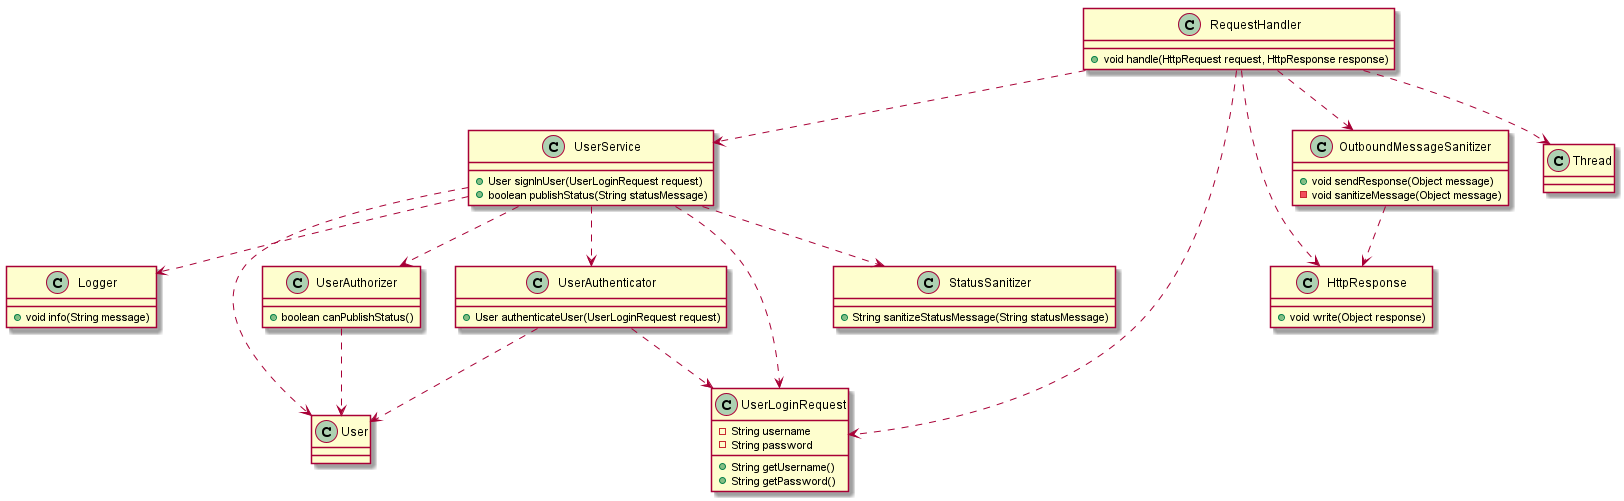
\includegraphics[width=\textwidth]{figure/ToyApp.png}
    \caption{Toy application.}
    \label{fig:toy_application}
\end{figure}

ArchUnit contains an extensive vocabulary for expressing typical architectural constraints. These constraints are typically composed of three parts. The first part indicates the type of Java construct that should be inspected. These constructs include classes, methods, fields and constructors. The second part contains a predicate that selects a subset of these constructs. The third part defines the condition that must hold true for all the selected constructs.

An example of a rule defined solely using this standard vocabulary can be seen in Listing~\ref{lst:standard_vocabulary}, where each of the three aforementioned parts of the constraint has been separated into their own line. The rule is a simple example of complete mediation, where some internal classes must only be accessed through a mediator.

\begin{minipage}{\linewidth}
\begin{lstlisting}[caption={Example of a rule that is expressed with the standard vocabulary.}, captionpos=b, label=lst:standard_vocabulary, numbers=left]
ArchRule rule = classes()
    .that().resideInAPackage("..internal..")
    .should().onlyBeAccessed().byAnyPackage("..mediator..");
\end{lstlisting}
\end{minipage}

In cases where this vocabulary is not sufficient for expressing a constraint, there is a possibility to define custom predicates and conditions over any given construct and supplying these as arguments to the \texttt{that()} and \texttt{should()} methods.

\subsection{Constraints}

\todo{Show rule definition for each constraint}
\todo{Show how each constraint is used in our toy app}

\subsubsection*{Log all security events}
This constraint is expressed with the assumption that there are services, in the form of one or several classes, that are responsible for performing security related events. Any publicly accessible method in these services must contain at least one call to the logging facility.

As seen in Listing~\ref{lst:constraint_1_impl}, the predicate that selects the security services, as well as the class responsible for logging, are passed as arguments to the architectural rule. This leaves no need for additional information in the source code.

\begin{minipage}{\linewidth}
\begin{lstlisting}[caption={Rule definition for constraint 1.}, captionpos=b, label=lst:constraint_1_impl, numbers=left]
ArchRule logSecurityEvents(
        DescribedPredicate<? super JavaClass> securityServicesDescriptor,
        Class<?> logger) {
    return methods()
        .that().haveModifier(JavaModifier.PUBLIC)
        .and().areDeclaredInClassesThat(securityServicesDescriptor)
        .should(callMethod(declaredIn(logger)));
}
\end{lstlisting}
\end{minipage}

\subsubsection*{Enforce AuthN/AuthZ at single point}
...

\begin{minipage}{\linewidth}
\begin{lstlisting}[caption={Rule definition for constraint 2.}, captionpos=b, label=lst:constraint_2_impl, numbers=left]
ArchRule enforceAuthenticationAtCentralPoint(
        Class<?> authenticationPoint,
        Class<?> authenticator) {
    return CompositeArchRule.of(
        theClass(authenticationPoint)
            .should(callMethod(declaredIn(authenticator)))
    ).and(
        methods()
            .that().areDeclaredIn(authenticator)
            .should(onlyBeAccessedBy(authenticationPoint))
    );
}
\end{lstlisting}
\end{minipage}

\subsubsection*{Every outbound message is sent from a central point of the system}
...

\begin{minipage}{\linewidth}
\begin{lstlisting}[caption={Rule definition for constraint 3.}, captionpos=b, label=lst:constraint_3_impl, numbers=left]
ArchRule sendOutboundMessagesFromCentralPoint(
        Class<?> sendingPoint,
        DescribedPredicate<? super JavaClass> senderDescriptor) {
    return CompositeArchRule.of(
        methods()
            .that().areDeclaredInClassesThat(senderDescriptor)
            .should(onlyBeAccessedBy(sendingPoint))
    ).and(
        fields()
            .that().areDeclaredInClassesThat(senderDescriptor)
            .should(onlyBeAccessedBy(sendingPoint))
    );
}
\end{lstlisting}
\end{minipage}

\section{With Additional Information in Code}

Some of the architectural constraints require that the developer injects additional information into the source code.

In some cases, this information is simply an indicator that says something about an entire class. Naming the class with a specific suffix is one approach to accomplish this. Another approach is to implement an empty interface, which is the technique used with Java's \texttt{Serializable}\footnote{https://docs.oracle.com/javase/7/docs/api/java/io/Serializable.html} interface. 

In other cases, however, the information may be required for methods of arbitrary signatures and even specific fields. For the purposes of flexibility and minimal obtrusiveness, any extra information is expressed in the form of annotations. These can be applied to classes, fields, methods and parameters without changing the underlying architecture of the system.

\todo{Specific example that requires additional information}

\subsection{Constraints}

\todo{Show rule definition for each constraint}
\todo{Show how each constraint is used in our toy app}

\subsubsection*{Input from a user is validated}
...

\begin{minipage}{\linewidth}
\begin{lstlisting}[caption={Rule definition for constraint 4.}, captionpos=b, label=lst:constraint_4_impl, numbers=left]
public static ArchRule validateUserInput() {
    return codeUnits()
        .that().areAnnotatedWith(UserInput.class)
        .should(performDirectOrIndirectValidation);
}
\end{lstlisting}
\end{minipage}

\subsubsection*{Allocation of resources is limited or throttled}
While resources is a broad term, this constraint focuses on preventing the exhaustion of CPU and memory resources through the creation of new threads and processes. As such, every block of code that contains a call to the \texttt{start()} method of a \texttt{Thread}\footnote{https://docs.oracle.com/javase/7/docs/api/java/lang/Thread.html} or any of its subclasses, must be marked as containing a resource restriction mechanism. The same rule is applied for calls to \texttt{ProcessBuilder.start()}\footnote{https://docs.oracle.com/javase/7/docs/api/java/lang/Process.html} and \texttt{Runtime.exec()}\footnotemark[3], which lead to the creation of new processes.
% TODO manual footnote, adjust as necessary

The marking is done with the help of an annotation, either on the relevant method or the entire class. The decision of how the restriction mechanism is implemented is left to the developer of the system.

\begin{minipage}{\linewidth}
\begin{lstlisting}[caption={Rule definition for constraint 5.}, captionpos=b, label=lst:constraint_5_impl, numbers=left]
public static ArchRule limitResourceAllocation() {
    return noClasses()
        .that().areNotAnnotatedWith(ResourceRestriction.class)
        .should().callMethodWhere(
            aThreadIsStartedWithoutRestriction
        ).orShould().callMethodWhere(
            aProcessIsStartedWithoutRestriction
        );
}
\end{lstlisting}
\end{minipage}

\section{With Extensions to ArchUnit}

In the current ArchUnit API, a rule that aims to constrain access to a method (or field) must be expressed in terms of the type signatures of the source and target methods. Some of our constraints require knowledge about the type signature of the object that is being passed as a parameter. This is a non-issue when fields and method parameters are of the same types as the objects being passed to them. However, in cases where a method signature accepts a "more general" type, such as an \texttt{Object}, there is no way for ArchUnit to constrain the types of the objects that are actually being passed as arguments.

ArchUnit builds its representation of the architecture using ASM\footnote{\url{https://asm.ow2.io/}}, a Java bytecode analysis framework. This framework contains functionality for keeping track of the stack and local variables while analyzing the instructions of a method. With knowledge of the type signatures of the references on the stack at the time of a method call or field assignment, it is possible to determine the type signatures of objects passed as method arguments or an object being assigned to a field. Our extension provides this additional information in ArchUnit's representation of accesses to fields and methods, which the rule definitions can then make use of.

\todo{Specific example that requires an extension}

\subsection{Extensions}

\todo{Detail the extensions we made}

\subsection{Constraints}

\todo{Show rule definition for each constraint}
\todo{Show how each constraint is used in our toy app}

\subsubsection*{Do not allow sensitive information to bleed to other components}
...

\subsubsection*{Do not log secrets}
...
